
\documentclass[a4paper,12pt]{article}

\usepackage[a4paper, total={6in, 8in}, left=30mm]{geometry}
\usepackage{pdfpages}

\usepackage{cmap}
\usepackage{caption}
\usepackage[T2A]{fontenc}
\usepackage[utf8]{inputenc}
\usepackage[english,russian]{babel}
\usepackage{fancyhdr}
\usepackage{minted}
\usepackage{hyperref}
\usepackage{amsmath}
\usepackage{graphicx}
\usepackage[document]{ragged2e}

\providecommand{\tightlist}{%
  \setlength{\itemsep}{0pt}\setlength{\parskip}{0pt}}

\hypersetup{
  pdfborderstyle={/S/U/W 1}
}

\graphicspath{./images/}

\pagestyle{fancy}
\fancyhf{}
\lhead{Антон Завьялов, ПИ-72}
\rhead{\textbf{Лабораторная №6}}
\cfoot{\thepage}

\makeatletter
\def\@seccntformat#1{%
  \expandafter\ifx\csname c@#1\endcsname\c@section\else
  \csname the#1\endcsname\quad
  \fi}
\makeatother

\begin{document}
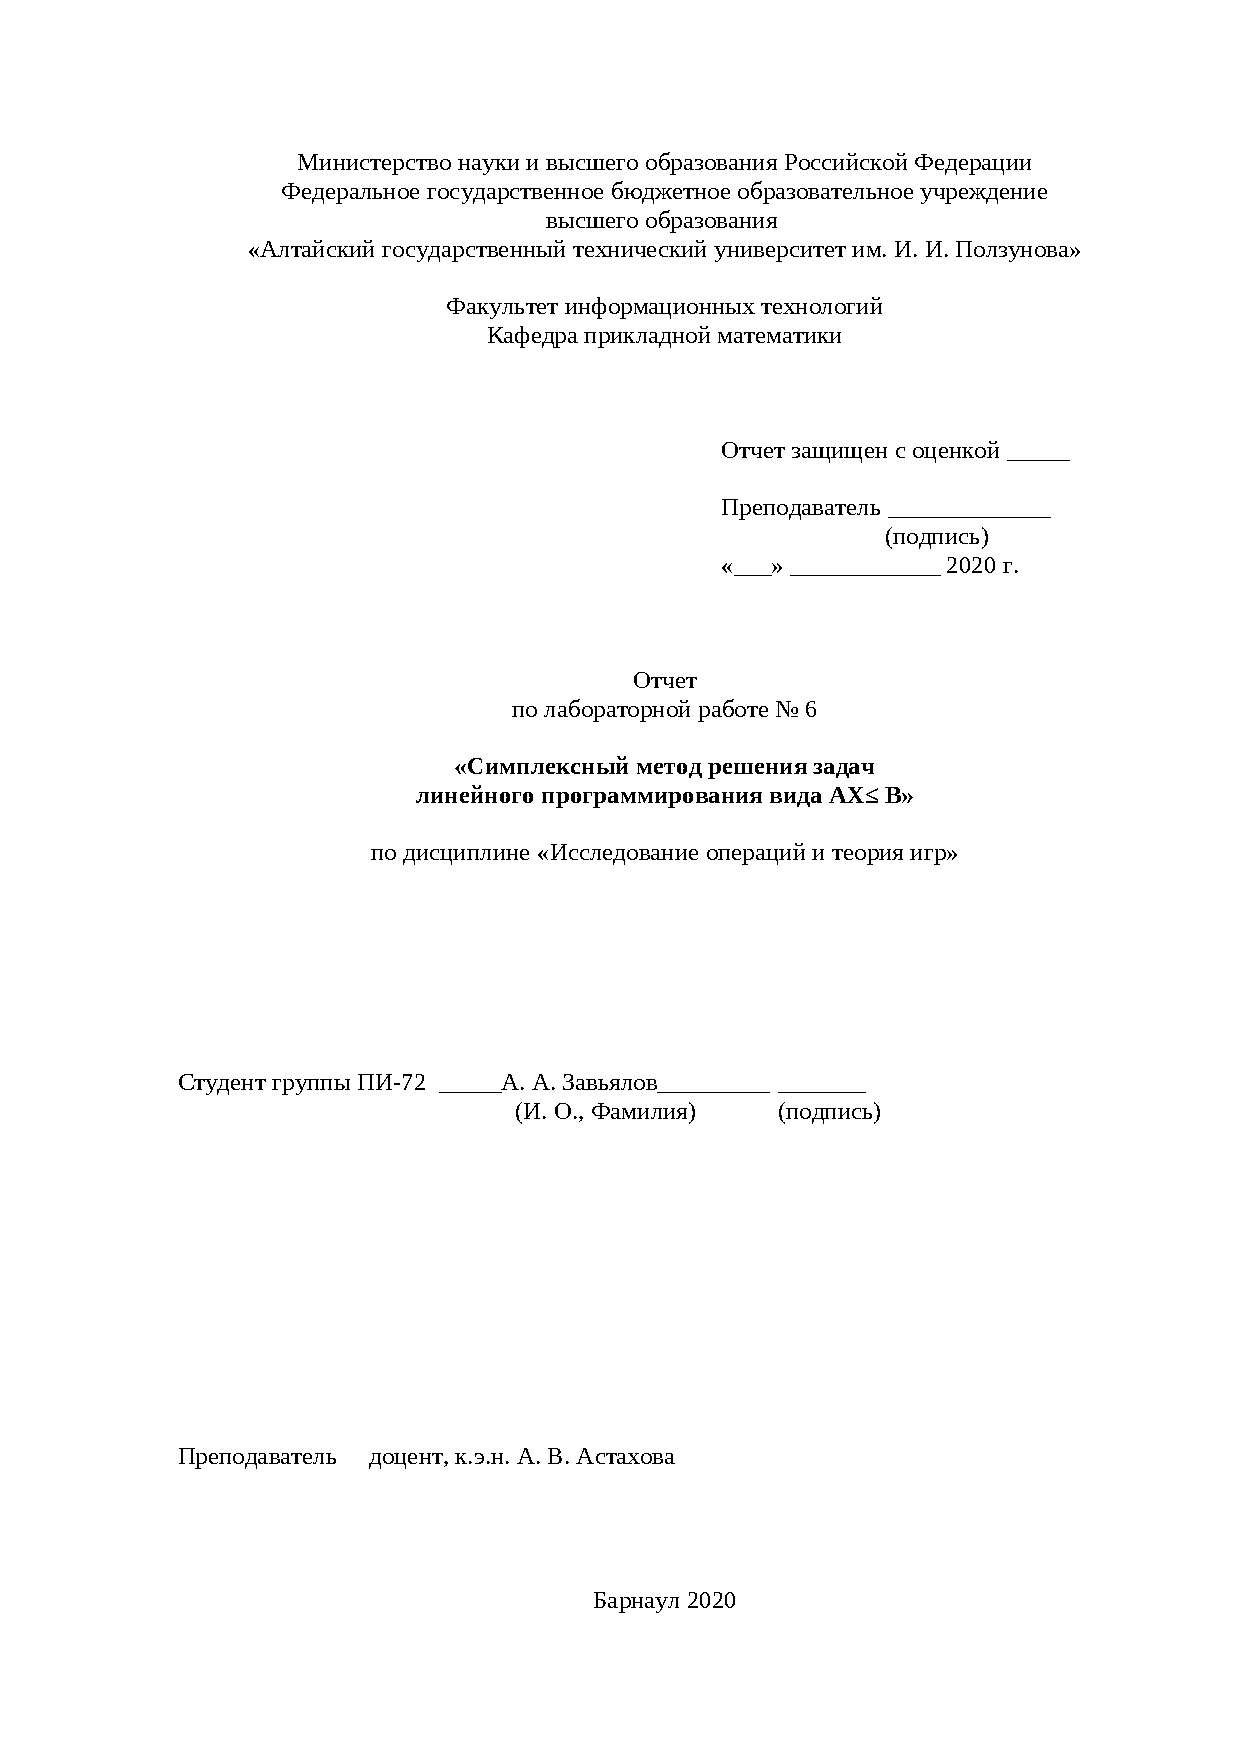
\includepdf[pages={1}]{title.pdf}

\section{\normalsize{Задание на лабораторную работу}}
\begin{flushleft}
\justify
\begin{enumerate}
\item
Используя теоретический материал по теме работы, в том числе, изложенный в Приложении  к данному заданию, повторить теоретические основы решения ЗЛП вида \textbf{AX $\le$ B} симплекс методом.
\item
    Используя тестовые примеры, разработанные на предыдущей лабораторной работе, разработать машинный алгоритм решения ЗЛП табличным симплекс-методом.\newline
    Составить и отладить программу решения ЗЛП вида $AX \le B$ симплекс методом на выбранном языке программирования. В программе не должно содержаться обращений к стандартным библиотекам, включающим процедуры реализации алгоритма симплекс-метода. Текст программы должен быть составлен студентом самостоятельно и включать \underline{подробные комментарии}, относящиеся к структурам данных и шагам алгоритма реализации симплекс метода.\newline
    Результат работы программы на каждом из тестовых примеров должен выводиться на экран монитора в виде:
    
    \textbf{Тест}: <условие теста>\newline
    \textbf{Оптимальное решение ЗЛП}: <min/max> F = <число>; X = ($x_1, x_2,$ $..., x_n$) = (<число>, <число>, ..., <число>); Z = ($z_1, z_2,$$..., z_m$) = (<число>,<число>,...,<число>).
\item
    Протестировать программу на необходимом количестве тестов, выявляющих логику работы всех ветвей программы.
\item
  Оформить отчет в текстовом редакторе, отправить преподавателю по электронной почте файл с отчетом на проверку преподавателю.
\end{enumerate}
\end{flushleft}

\pagebreak

\section{\normalsize{Выполнение работы. Исходный текст программы}}
\begin{flushleft}
\justify
Исходный код ПО на языке программирования \textbf{Scala} и код отчёта в системе вёртски \LaTeX $~$ доступен по ссылке: \url{https://github.com/andiogenes/iso/tree/master/lab_6}.\newline\linebreak
\textbf{Main.scala}
\inputminted[breaklines]{scala}{../src/main/scala/Main.scala}
\end{flushleft}

\pagebreak

\section{\normalsize{Результаты тестирования программы}}
\begin{flushleft}
\justify
\begin{figure}[H]
  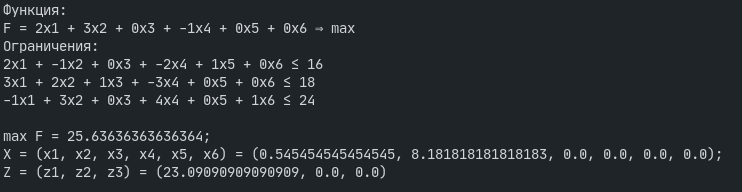
\includegraphics[width=12.25cm,height=3.5cm]{images/output1.png}
  \centering
  \caption{Задача из прошлой работы}
\end{figure}
\begin{figure}[H]
  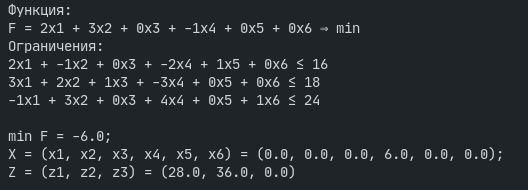
\includegraphics[width=10.25cm,height=3.5cm]{images/output2.png}
  \centering
  \caption{}
\end{figure}
\begin{figure}[H]
  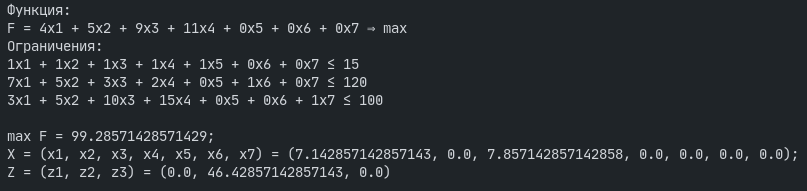
\includegraphics[width=12.25cm,height=3.5cm]{images/output3.png}
  \centering
  \caption{}
\end{figure}
\begin{figure}[H]
  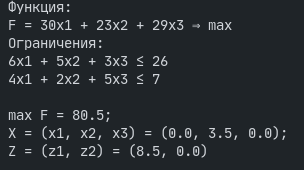
\includegraphics[width=6.25cm,height=3.5cm]{images/output4.png}
  \centering
  \caption{}
\end{figure}
\begin{figure}[H]
  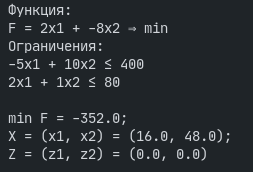
\includegraphics[width=6.25cm,height=3.5cm]{images/output5.png}
  \centering
  \caption{}
\end{figure}
\begin{figure}[H]
  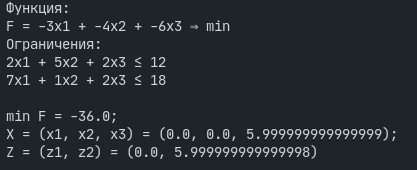
\includegraphics[width=8.25cm,height=3.5cm]{images/output6.png}
  \centering
  \caption{}
\end{figure}
\end{flushleft}

\end{document}
